%!TEX TS-program = xelatex
\documentclass[12pt,a4paper]{report}
\usepackage[utf8]{inputenc}
\usepackage{dirtree}
\usepackage{listings}
\usepackage{color}
\usepackage{fancyhdr}
\usepackage{titlesec, blindtext, color}
\usepackage{amsmath}
\usepackage{graphicx}
\usepackage{csvsimple}
\usepackage{url}
\usepackage{hyperref}
\usepackage{booktabs}
\usepackage{tabularx}
\usepackage[margin=0.8in]{geometry}
\usepackage{float}
\usepackage{subfig}
\usepackage{listings}
\usepackage{upgreek}
\usepackage[american]{circuitikz}
\usepackage[titletoc,title]{appendix}
\usepackage{amssymb}
\usepackage{array,etoolbox}
\usepackage[parfill]{parskip}
\usepackage{ragged2e}
\usepackage{pgfplots}
\usepackage{pdfpages}
\usepackage{svg}
\usepackage{lastpage}
\usepackage{xcolor}
\hypersetup{
    colorlinks,
    linkcolor={red!50!black},
    citecolor={blue!50!black},
    urlcolor={blue!80!black}
}
\pgfplotsset{width=10cm,compat=1.9} 
\usepgfplotslibrary{external}
\tikzexternalize 

\newcommand{\hsp}{\hspace{20pt}}
\titleformat{\chapter}[hang]{\Huge\bfseries}{\thechapter\hsp}{0pt}{\Huge\bfseries}

\preto\tabular{\setcounter{magicrownumbers}{0}}
\newcounter{magicrownumbers}
\newcommand\rownumber{\stepcounter{magicrownumbers}\arabic{magicrownumbers}}
\newcommand{\ruler}{\noindent\rule{\textwidth}{1pt}}

% Standard colors for the code syntax highlighting.
\definecolor{pblue}{rgb}{0.13,0.13,1}
\definecolor{pgreen}{rgb}{0,0.5,0}
\definecolor{pred}{rgb}{0.9,0,0}
\definecolor{pgrey}{rgb}{0.46,0.45,0.48}

\def\doubleunderline#1{\underline{\underline{#1}}}
\newcommand{\doubleindent}{\indent \indent}

% Define Y colymntype
\newcolumntype{Y}{>{\centering\arraybackslash}X}

\definecolor{mygreen}{rgb}{0,0.6,0}
\definecolor{mygray}{rgb}{0.5,0.5,0.5}
\definecolor{mymauve}{rgb}{0.58,0,0.82}

\lstset{ 
  backgroundcolor=\color{white},   % choose the background color; you must add \usepackage{color} or \usepackage{xcolor}; should come as last argument
  basicstyle=\footnotesize,        % the size of the fonts that are used for the code
  breakatwhitespace=false,         % sets if automatic breaks should only happen at whitespace
  breaklines=true,                 % sets automatic line breaking
  captionpos=b,                    % sets the caption-position to bottom
  commentstyle=\color{mygreen},    % comment style
  deletekeywords={...},            % if you want to delete keywords from the given language
  escapeinside={\%*}{*)},          % if you want to add LaTeX within your code
  extendedchars=true,              % lets you use non-ASCII characters; for 8-bits encodings only, does not work with UTF-8
  frame=single,	                   % adds a frame around the code
  keepspaces=true,                 % keeps spaces in text, useful for keeping indentation of code (possibly needs columns=flexible)
  keywordstyle=\color{blue},       % keyword style
  language=C,                      % the language of the code
  numbers=left,                    % where to put the line-numbers; possible values are (none, left, right)
  numbersep=5pt,                   % how far the line-numbers are from the code
  numberstyle=\tiny\color{mygray}, % the style that is used for the line-numbers
  rulecolor=\color{black},         % if not set, the frame-color may be changed on line-breaks within not-black text (e.g. comments (green here))
  showspaces=false,                % show spaces everywhere adding particular underscores; it overrides 'showstringspaces'
  showstringspaces=false,          % underline spaces within strings only
  showtabs=false,                  % show tabs within strings adding particular underscores
  stepnumber=1,                    % the step between two line-numbers. If it's 1, each line will be numbered
  stringstyle=\color{mymauve},     % string literal style
  tabsize=4,	                   % sets default tabsize to 2 spaces
  title=\lstname                   % show the filename of files included with \lstinputlisting; also try caption instead of title
}

% Group name
\newcommand{\groupname}{Group}

% Define author information
\newcommand{\authors}{Philip Hjortsberg, William Wennerström}
\newcommand{\authorsinfo}{
    Hjortsberg, Philip\\
    \texttt{\href{
        mailto:phihjo-2@student.ltu.se
    }{\color{black}{
        phihjo-2@student.ltu.se
    }}}
    
    \and
    
    Wennerström, William\\
    \texttt{\href{
        mailto:wenwil-5@student.ltu.se
    }{\color{black}{
        wenwil-5@student.ltu.se
    }}}
}

% Define course information
\newcommand{\coursename}{Design of Dynamic Web Systems}
\newcommand{\coursecode}{M7011E}

% Define project name
\newcommand{\projectname}{Project Roaster}

% Define information about the school/university
\newcommand{\schoolinfo}{Department of Computer Science, \\
                         Electrical and Space Engineering \\
                         \bigskip{}
                         Luleå University of Technology \\
                         Luleå, Sweden
}

\title{
    \coursecode{} \\
    \coursename{} \\
    \vspace{1.8em}
    \textbf{\projectname{}} \break
    \author{
        \authorsinfo{}
    } \break{}
    \schoolinfo{}}
\renewcommand\footnotemark{}
    \date{\today}
 
\pagestyle{fancyplain}
\renewcommand{\headrulewidth}{0pt}
\renewcommand{\footrulewidth}{0pt}
\lhead{}
 
\begin{document}

\maketitle
\thispagestyle{empty} % Disable page numbers for this page.
\newpage

{\hypersetup{linkcolor=black}
    \tableofcontents}
\newpage

\chapter{The problem}
One of the big pains when programming in groups is code that is unreadable. Many times you can look at a code snippet and see who wrote that piece
just based on the formatting and comments. The solution to this is to enforce a uniform code and documentation style that every person adheres to.
This is normally done by installing a linting tool chain and configuring it equally on all systems used for developing. 
The idea for this project is to eliminate the installing and configuring step by doing it all in the site called Roaster, along with the intriguing feature of following your own and friends code quality progress.

Roast analyzes and grades your code. The user can register and follow their personal programming progress and compare it with people you follow! 
You could compare it to music scrobbling, but for code.
Personal statistics is generated by running static code analysis on the uploaded code - data such as number of errors, number of warnings and even code style problems is collected.
The statistics can then be viewed in a feed where both your own and your friends progress is listed.
Global statistics like most common errors and number of rows analyzed is displayed on a page that can be viewed by everyone.

\chapter{System design}

\chapter{System architecture}
The system architecture is designed to be deploy able independently of underlying platform. This led us to containerize the server in order to facilitate the deployment process and avoid installation mishaps. Both the databases are not containerized as there is no gain in doing so.
The whole architecture is intended to be scalable as implemented right now in Amazon Web Services (AWS). If the solution is to be deployed at some other hosting solution like your own servers, and scalability is wanted, one would need to implement an load balancer in front of all the application servers. It's also wise to setup a heavily tested reverse proxy on the load balancer, like nginx and setup the TLS certificates here. To match the size of your application server you would maybe like to scale the databases. Since these to not run in docker or with any special configurations, it should be easy to just follow standard best practices for clustering Redis and PostgreSQL.
The communication between the application server and the databases are not encrypted as of now since they are all hosted in a Virtual Private Cloud (VPC) in AWS and thereby sandboxed. If implementing this on your own data centre or hardware you have to decide on this your self in order to secure the architecture. The application server has support for encrypted communication between both databases. 

The flake8 component that analyzes Python code is executed in the same docker as the application server. This is safe since the flake8 analyzer does not run any code, only parses it.
The application server has access to local system calls and can thereby start the analyzer. The communication back from the analyzer is encoded in JSON which is very convenient for web application.

The front end is based on a JavaScript framework called Mithril.js that encourages modularization and a model component based pattern. This takes advantage of a virtual DOM that utilizes diffing which makes it very fast, and mitigates many security risks like XSS attacks. 

\begin{figure}[H]
  \centering
  \includesvg[width=16cm]{architecture.svg}
  \caption{High level system architecture overview.}
\end{figure}
\chapter{Application Programming Interface}
\chapter{Technology choices}
The participants of the course were encouraged to learn new technologies and tools that the developers had never used before or wanted to learn more about. The technologies chosen all was chosen with scalability and security in mind, whenever applicable the developers chose enterprise grade software.
\section{Database}
In order to choose the right database for a project the designers need to consider what type of data that is to be stored and if availability (NoSQL) or robustness(SQL) is of utmost importance.
Considering the aspects above the developers chose robustness, an SQL database should be the best choice for this type of application where mainly structured data is stored. 
While designing the system, the developers wanted the database to handle objects, hence a Object Relational Database (ORD) was desired and PostgreSQL has good support for advanced features for object handling and custom definition of objects. PostgreSQL is also fully ACID compliant which is desired. PostgreSQL has the ability to use advanced constraints which enables better robustness. PostgreSQL also has support for the complete official SQL syntax. PostgreSQL is the most advanced and fastest DB\cite{db-benchmark} that is free to use and open source.
One of the two developers in this project has prior experience with PostreSQL but only shallow knowledge which also made it interesting as a technology to learn more about.

One of the advanced features PostgreSQL has is it's \texttt{HSTORE}, the ability to store sets of key/value pairs within a single PostgreSQL value. During the design phase the developers thought this feature would be good to have when storing the "Roasts" but as it turns out, it was not necessary.

Competing technologies that we discarded due to the following drawbacks.
\begin{itemize}
    \item MySQL is not fully ACID compliant, ignores \texttt{check} commands.
    \item SQLite doesn't scale and is weakly typed.
    \item MariaDB doesn't offer the same amount of data integrity out of the box, up to the user to implement it correctly. 
\end{itemize}

\section{Session Database}
To check sessions in a speedy fashion a fast in memory key/value database is used. The choice is Redis, an advanced software made for horizontal scaling by clustering. It's superior to Memcached in key names, whereas Memchached only supports 250 bytes of plain strings, Redis handles key/values to be as big as 512MB and any kind of binary data. Redis is also more modern and up to date which makes it more popular and a more relevant technology to learn.

\section{Containerized Server}
A server housed in a docker container makes deployment very simple, just swap the container with the new one! This also makes it easier to deploy the application on a different cloud, in a development environment or on dedicated hardware. Docker also works good in a CI/CD solution which we employ.

\section{Golang Server}
To acquire more in depth knowledge of a web servers inner workings we chose to write the server without a framework. The language of choice is Golang since it has a solid foundation as a web server language and that one of the developers had prior experience with it being good at handling network traffic with just the built in \texttt{http/net} package. To facilitate faster development and to not have to to everything from scratch the developers chose to use an existing back end router built in go, called \texttt{Gorilla}.
The Go language also has good support for connecting to databases such as those above which eases development. 

\section{Hosting Platform}
To have a good uptime and availability the solution needs to be deployed on a platform that supports these constraints. The developers had the following possibilities:

\begin{itemize}
    \item To host on personal hardware in a student maintained data center called LUDD. This would ensure that enough resources are available for the application since the hardware is decent. Potential downside was the uptime, the facility has recently had problems with stability which is a major factor.
    \item To host on Virtual Machine provided by LUDD, as previously stated the stability is a major factor and therefore not used.
    \item Cloud infrastructure, due to the fact that the authors are students, they had access to various cloud solutions for free and due to that cloud based experience is valued in the market today, the choice was made to implement the solution in the cloud.
\end{itemize}

Choosing the cloud platform is not easy, determining if you want PaaS, IaaS or some hybrid took a while. In the end it came down to maturity, scalability and where we had enough credits to run our solution. Amazon Web Services offers a solution called elastic beanstalk which is a hybrid PaaS with automatic scaling which is used as the platform for the application. The server in the docker container resides in an AWS EC2 instance, which is a IaaS. The databases are hosted in Amazon Relational Database Service (RDS) which is SaaS. 

Amazon Elastic beanstalk also incorporates a elastic load balancer which is what makes scaling really simple when using multiple application servers. 

Due to the technology choices being deliberately chosen to be platform independent, a change of cloud provider or move to physical hardware would not be an impossible task.
\section{Front end Framework}
The website will not be very big when it comes to number of pages and views.
The desired outcome of the project is a website that feels fast as well as secure, based on modern technologies. When accessing a website, your browser start by downloading the defined files, and the website ill load faster if those files are smaller. Hence we wanted a small framework.
We could have written the website with pure \textit{vanilla} JavaScript but frameworks most often makes things easier for the developers by not needing to write a frontend router. Other reasons to choose a framework is Virtual DOM, separate API from frontend and to learn how to write a Single Page Application.

Considered technologies was the following:
\begin{itemize}
    \item React.js + Redux router, was a good candidate with a Virtual DOM, good community support and neither of the developers had written in it before. Down side was the size of React.js together with Redux.
    \item Vue.js also has a virtual DOM and good community support, but is big in size.
    \item Angular.js Does not have a virtual DOM and does therefore not qualify for our needs.
    \item Mithril.js Has a virtual DOM, is small in size and it's virtual DOM is fastest of the ones listed above. Smaller community but suits the needs of the project and is therefore chosen.
\end{itemize}

\chapter{Description of software parts and interaction between them}

\newpage

\chapter{Security considerations}
Several security issues has been taken into consideration when developing the system.

\section{HTTPS/TLS}
The connection from the client to the web server is made over TLS with a Amazon signed certificate.
This is configured by the Elastic Load Balancer running on Elastic Beanstalk that acts like a reverse proxy.
The request then propagates through our VPC (Virtual Private Cloud) in AWS in plaintext. 

\section{CSRF}
\label{subsec:csrf}
The site has implemented protection against CSRF (Cross Site Request Forgery). CSRF is a man-in-the-middle attack where the automatic cookie submission (the cookie is always sent for every request by the web browser) is abused. A site that utilizes cross-origin requests cannot use the \texttt{site-only} attribute for cookies, i.e. another malicious website open in another tab can also issue authenticated requests to the web service\cite{rick}.

In order to increase the security against CSRF attacks we have chosen to use and implement a rolling random token scheme. The rolling scheme will ensure that the CSRF token is not stolen as demonstrated by the BREACH attack\cite{breach}. First, a CSRF cookie is issued by the web server to sign challenges against, then a challenge is issued by the web server as a HTTP header called \texttt{X-CSRF-Token} for every request.

We also had to implement our own network handling when using XHR requests in the frontend due to the CSRF mitigation system. The library we have implemented, called \texttt{Network}\cite{roaster-network}, wraps the Mithril.js \texttt{m.request} method and retrieves the new \texttt{X-CSRF-Token} header for every requests and then saves it so it can be used for the next XHR request.

All HTTP methods, except \texttt{GET, HEAD, OPTIONS} and \texttt{TRACE}, that are sent to the web server are required to authenticate with the CSRF challenge response mechanism. Therefore the \texttt{Network} library creates a \texttt{HEAD} request toward the \texttt{/} (root) API endpoint to receive the first initial \texttt{X-CSRF-Token} for the rolling scheme.

Cookie security that can mitigate XSS attacks is discussed below in \hyperref[subsec:secure-cookies]{Security considerations - Secure cookies}.

\section{XSS}
The Mithril.js framework will automatically escape all HTML tag characters before inserting into the Virtual DOM that it creates\cite{mithril-trust}. Therefore most XSS (Cross Site Scripting) issues are mitigated. However, because we also use jQuery which \textit{does not} escape HTML tag characters, the escaping is done explicitly for the search bar component.

Removing the jQuery dependency is discussed in the \hyperref[subsec:remove-jquery]{Future work - Remove jQuery} section below.\\
Cookie security that can mitigate XSS attacks is discussed below in \hyperref[subsec:secure-cookies]{Security considerations - Secure cookies}.

\section{Secure cookies}
\label{subsec:secure-cookies}
User session cookies is stored in the cookie store in the browser. These are validated with the HMAC verification mechanism and encrypted with AES-256. HMAC verification ensures that the cookie content has not been tampered with during the transfer\cite{fips-198}. While AES-256 encrypts the data contained within the cookie, ensuring that no one can read it\cite{fips-197}. Even with TLS these are real issues due to the BREACH/CRIME vulnerability that is able to extract the HTTP headers for encrypted transfers\cite{breach}. The BREACH attack is mitigated using the rolling CSRF token scheme explained above in \hyperref[subsec:csrf]{Security considerations - CSRF}

The session cookies has the \texttt{HttpOnly} attribute enabled which sandboxes the cookie so it cannot be accessed by JavaScript. This will mitigate the most common XSS attacks\cite{owasp-httponly}. Additionally the \texttt{sameSite} attribute is set to \texttt{Strict} which tells the browser that it should not send the cookie with cross-site requests\cite{owasp-samesite}. The \texttt{sameSite} attribute will mitigate CSRF attacks, but is only supported in modern browsers. As of August 2018 only $68,92 \%$ of the browsers used by Internet users supports the \texttt{sameSite} attribute\cite{owasp-samesite-support}. We concluded that this low adoption is reason enough to implement the rolling CSRF token scheme described above.

\section{Password storage}
There are a lot of challenges keeping user credentials secured. Our solution is based on well known algorithms, Bcrypt and SHA-512. The implementation uses official libraries in Go, the language in which the server is written, so that we don't make the mistake of "rolling our own crypto".

The plaintext password that is provided by the user will first be transformed to a hash sum with SHA-512. This is due to that Bcrypt limits the input to 72 bytes. By hashing the password with SHA-512 more entropy of the original password is kept. Also, some implementations of Bcrypt that allows for longer passwords can be vulnerable to DoS attacks\cite{bcrypt-length}.

The SHA-512 hash sum is then hashed again using Bcrypt. This is because
SHA-512 is a \textit{fast} hash algorithm not made for password hashing. Bcrypt is
designed to be slow and hard to speed up using hardware such as FPGAs and
ASICs. The work factor is set to 12 which should make the expensive Blowfish
setup take $> 250$ ms ($364.815906$ ms precisely on one of our laptops).
The Bcrypt algorithm also takes care of salting of the password and prepends 
it with the resulting hash.

Dropbox has a great article\cite{dropbox-passwords} on their password hashing scheme which our
scheme shares many similarities with, we do not, however, use AES-256 with a
global pepper (shared global encryption key) which is overkill for our use
case. They also encode their SHA-512 with base 64, which is not needed in our
case because we can save the hash as raw bytes (PostgreSQL's \texttt{bytea}).

Some implementations of Bcrypt uses a null byte (\texttt{0x00}) to determine the end
of the input\cite{bcrypt-bug}, the Go implementations does \textit{not} have this problem. So there
is no need to encode the data as base 64. This is verified using the program that was created for
this project in the \texttt{cmd/testbcrypt} source folder.

The approach used by Dropbox where they encode with base $64$ will generate a
$\approx 88$ byte long key, which is then truncated to $72$ bytes. This results in a
input with $64^{72}$ possible combinations. Our approach of not encoding the
input as base $64$ results in a $64$ byte long key (the output size of SHA-512),
where there is 256 possible combinations \textit{per byte}. This results in an input
with $256^{64}$ possible combinations. Therefore our approach allows for far more
possible entropy because $64^{72} \ll 256^{64}$ ($\approx 1,2 \times 10^{24}$ times more!).

The amount of possible entropy for both solution is so high that comparing the differences
between them two doesn't really make sense - but our solution that allows for more entropy
\textit{also} skips the unnecessary base 64 encode step due to the lack of the null byte bug.

\chapter{Discussion}
The \texttt{analyze/...} package that was written in Go for this project should be easy to extend and uses a generic interface. Also, the cache in \texttt{analyze/cache/...} is custom built for Roaster's use case and is made to be able to handle any code result.

\section{Cloud provider}
In hindsight, we might have chosen a different cloud provider due to complexity in the configuration and maintaining of the service. TODO FILL WITH MORE INFO
\chapter{Future work}
\label{sec:future-work}
The proof of concept is finished for Roaster and the service works as we wanted, but there are several ways to extend the service and improve it. Below follows some larger changes that could extend Roaster. Additionally the current issues that should be solved before extending Roaster is presented in the \hyperref[sec:issue-tracker]{Future work - Issue tracker} section.

\section{More languages}
One of the more obvious improvements is to add more languages than Python 3. A simple start would be to add Python 2.7. An interface for each language's static analyze toolkit has to be implemented that can fulfill the \texttt{analyze/...} package's generic \texttt{RoastResult} interface. Adding other languages than Python should be easy, but requires that a new toolchain and environment is setup for that specific language on the same system as the web service is running.

\section{Microservices}
To ensure that the service can scale as it grows the analyze system could be split into separate microservices for every language. Even in its current implementation a cache is required due to the slowness of the static analysis tools. Microservices would greatly reduce the load on the main web services. The microservice would communicate using a message queuing system, e.g. RabbitMQ, where the main web services can publish a new request and get a response later from one of the microservices. These microservices would be easy to scale for user demand.

\section{Statistics}
The presentation and collection of statistics could need more work so that more relevant statistics is presented to the user. An easy start would be statistics for the type of errors and warnings - the data already exists in the backend but is not compiled together for easy parsing through the REST API.

\section{CLI and IDE integration}
REVOLUTION!!!!!!!

\section{Issue tracker}
\label{sec:issue-tracker}
\textbf{\textsuperscript{F}} Requires frontend changes. \\
\textbf{\textsuperscript{B}} Requires backend changes.

\subsection*{Enhancements}
\subsubsection{Remove jQuery\texorpdfstring{\textsuperscript{F}}{}}
\label{subsec:remove-jquery}
jQuery is used for the search feature and was added due to time constraints, in the future the search component can be implemented with Mithril.js and the jQuery dependency can be removed, thus removing the overhead of having to mitigate XSS injections for non-Mithril.js components.

Tracked in issue: \href{https://github.com/LuleaUniversityOfTechnology/2018-project-roaster/issues/225}{\#225}

\subsubsection{Refactor UserModel\texorpdfstring{\textsuperscript{F}}{}}
The logged in user's data is saved in the static \texttt{UserModel} model. It would be better to have a object that is passed to the views that require them (composition), this would allow for merging the \texttt{Profile} and \texttt{User} views for more DRY code. Additionally the request methods should be moved into the model to prevent code duplication. The statistics models are already implemented like this and can be used as insperation.

Tracked in issue: \href{https://github.com/LuleaUniversityOfTechnology/2018-project-roaster/issues/184}{\#184}

\subsubsection{Use LESS instead of overriding CSS through Mithril.js\texorpdfstring{\textsuperscript{F}}{}}
The Semantic UI styling framework is used for most of the styling of the views. In some cases the definitions by Semantic UI is overrided inline through Mithril.js. Later during the project the \texttt{semantic-ui-less} package was pulled in and integrated with the Webpack build environment. Most of the inline CSS definitions can be removed and be defined as LESS that is compiled together with Semantic UI instead.

Tracked in issue: \href{https://github.com/LuleaUniversityOfTechnology/2018-project-roaster/issues/130}{\#130}

\subsubsection{Clean up error handling\texorpdfstring{\textsuperscript{F}}{}}
There is no clear error handling pattern used for the frontend. The situation has gotten better throughout the project but there are still some parts of the code base that do not handle errors in a nice way.

Tracked in issue: \href{https://github.com/LuleaUniversityOfTechnology/2018-project-roaster/issues/115}{\#115}

\subsection*{Features}
\subsubsection{View specific Roast result\texorpdfstring{\textsuperscript{F+B}}{}}
After a user has been Roasted their submission is saved in the database, but they cannot view their code later when they have closed the page. A feature where they can view their previous results would be a great addition to view their progress.

This would require us to implement new API endpoints and also create a new view with the Monaco editor.

Tracked in issue: \href{https://github.com/LuleaUniversityOfTechnology/2018-project-roaster/issues/163}{\#163}

\subsection*{Bugs}
\subsubsection{Fix overflow for Roast submission messages\texorpdfstring{\textsuperscript{F}}{}}
There is an issue where the scrollbar doesn't appear when the Roast submission messages overflow. This happens when the user submits code with many errors and/or warnings.

Tracked in issue: \href{https://github.com/LuleaUniversityOfTechnology/2018-project-roaster/issues/134}{\#134}

\subsubsection{Register XHR request callback gets interrupted by Google  Chrome\texorpdfstring{\textsuperscript{F}}{}}
With a cold browser cache the XHR request callback gets interrupted by Google Chrome. This is \textit{probably} due to the 6 max TCP connections limit in the web browser. This bug only occurs for Google Chrome with a cold cache, if the cache is warm there is no issues.

The interrupt will stop Mithril.js from redirecting to the front page upon a successful registration. The user registration is correctly registered by the backend and the user is still able to login with the newly created account.

Tracked in issue: \href{https://github.com/LuleaUniversityOfTechnology/2018-project-roaster/issues/226}{\#226}

\subsubsection{Requirement for full name differs with the backend\texorpdfstring{\textsuperscript{F}}{}}
Upon registration the user is required to fill in their full name, even though it's not a requirement in the backend. Several views in the frontend utilizes the full name and they should be updated to show the username if there is not full name defined.

The registration requirement for a full name can be removed after the views has been updated.

Tracked in issue: \href{https://github.com/LuleaUniversityOfTechnology/2018-project-roaster/issues/210}{\#210}

\newpage
\apptocmd{\sloppy}{\hbadness 10000\relax}{}{} 
{\RaggedRight\begin{thebibliography}{1}

\bibitem{rick}
Ramgattie, R (2018, May 14) {\em  Cracking Java’s RNG for CSRF - Javax Faces and Why CSRF Token Randomness Matters.}
Fetched 2019-01-10, from:
\url{https://blog.securityevaluators.com/cracking-javas-rng-for-csrf-ea9cacd231d2}.

\bibitem{breach}
Gluck, Y., Harris N., \& Prado A. (2013, July 12) {\em BREACH: Reviving the Crime Attack, pp. 3, 11.} \\
Fetched 2019-01-10, from:
\url{http://breachattack.com/resources/BREACH%20-%20SSL,%20gone%20in%2030%20seconds.pdf}

\bibitem{roaster-network}
LuleaUniversityOfTechnology/2018-project-roaster (2019) {\em 2018-project-roaster/network.ts at 19529..28560.}
Fetched 2019-01-10, from:
\url{https://github.com/LuleaUniversityOfTechnology/2018-project-roaster/blob/1952964/www/src/services/network.ts#L38}.

\bibitem{mithril-trust}
Mithril.js 2.0.0-rc3 (2018) {\em trust(html) - Mithril.js}
Fetched 2019-01-10, from:
\url{https://mithril.js.org/trust.html#how-it-works}

\bibitem{fips-198}
NIST (2002, March 2) {\em FIPS 198-1, The Keyed-Hash Message Authentication Code (HMAC), p. 1.} \\
Fetched 2019-01-10, from:
\url{https://ia902804.us.archive.org/2/items/DTIC_ADA401868/DTIC_ADA401868.pdf}

\bibitem{fips-197}
NIST (2001, November 26) {\em FIPS 197, Annoucing the Advanced Encryption Standard (AES), p. 5.} \\
Fetched 2019-01-10, from:
\url{https://ia802809.us.archive.org/0/items/DTIC_ADA403903/DTIC_ADA403903.pdf}

\bibitem{owasp-httponly}
OWASP (2017) {\em HttpOnly.} Fetched 2019-01-11, from:
\url{https://www.owasp.org/index.php/HttpOnly}

\bibitem{owasp-samesite}
OWASP (2017) {\em SameSite.} Fetched 2019-01-11, from:
\url{https://www.owasp.org/index.php/SameSite}

\bibitem{owasp-samesite-support}
OWASP (2017) {\em Cross-Site Request Forgery (CSRF) Prevention Cheat Sheet.} Fetched 2019-01-11, from:
\url{https://www.owasp.org/index.php/Cross-Site_Request_Forgery_(CSRF)_Prevention_Cheat_Sheet#Samesite_Cookie_Attribute}

\bibitem{bcrypt-length}
Goodin, D (2013, September 16) {\em Long passwords are good, but too much length can be a DoS hazard} \\
Fetched 2019-01-10, from:
\url{https://arstechnica.com/information-technology/2013/09/long-passwords-are-good-but-too-much-lenghttps://www.overleaf.com/project/5c373ca83d7cdc5c90606ef4th-can-be-bad-for-security/}

\bibitem{dropbox-passwords}
Akhawe, D. (2016, September 21) {\em How Dropbox securely stores your passwords} \\
Fetched 2019-01-10, from:
\url{https://blogs.dropbox.com/tech/2016/09/how-dropbox-securely-stores-your-passwords/}

\bibitem{bcrypt-bug}
Ferrara, A (2015, March 12) {\em Security Issue: Combining Bcrypt With Other Hash Functions} \\
Fetched 2019-01-10, from:
\url{https://blog.ircmaxell.com/2015/03/security-issue-combining-bcrypt-with.html}

\bibitem{db-benchmark}
Castillo, J (2018) {\em PostgreSQL vs MySQL vs MariaDB - Help me Decide} \\
Fetched 2019-01-11, from:
\url{https://stackshare.io/stackups/mariadb-vs-mysql-vs-postgresql}

\end{thebibliography}}

\begin{appendix}
\chapter{Setup and install manual}
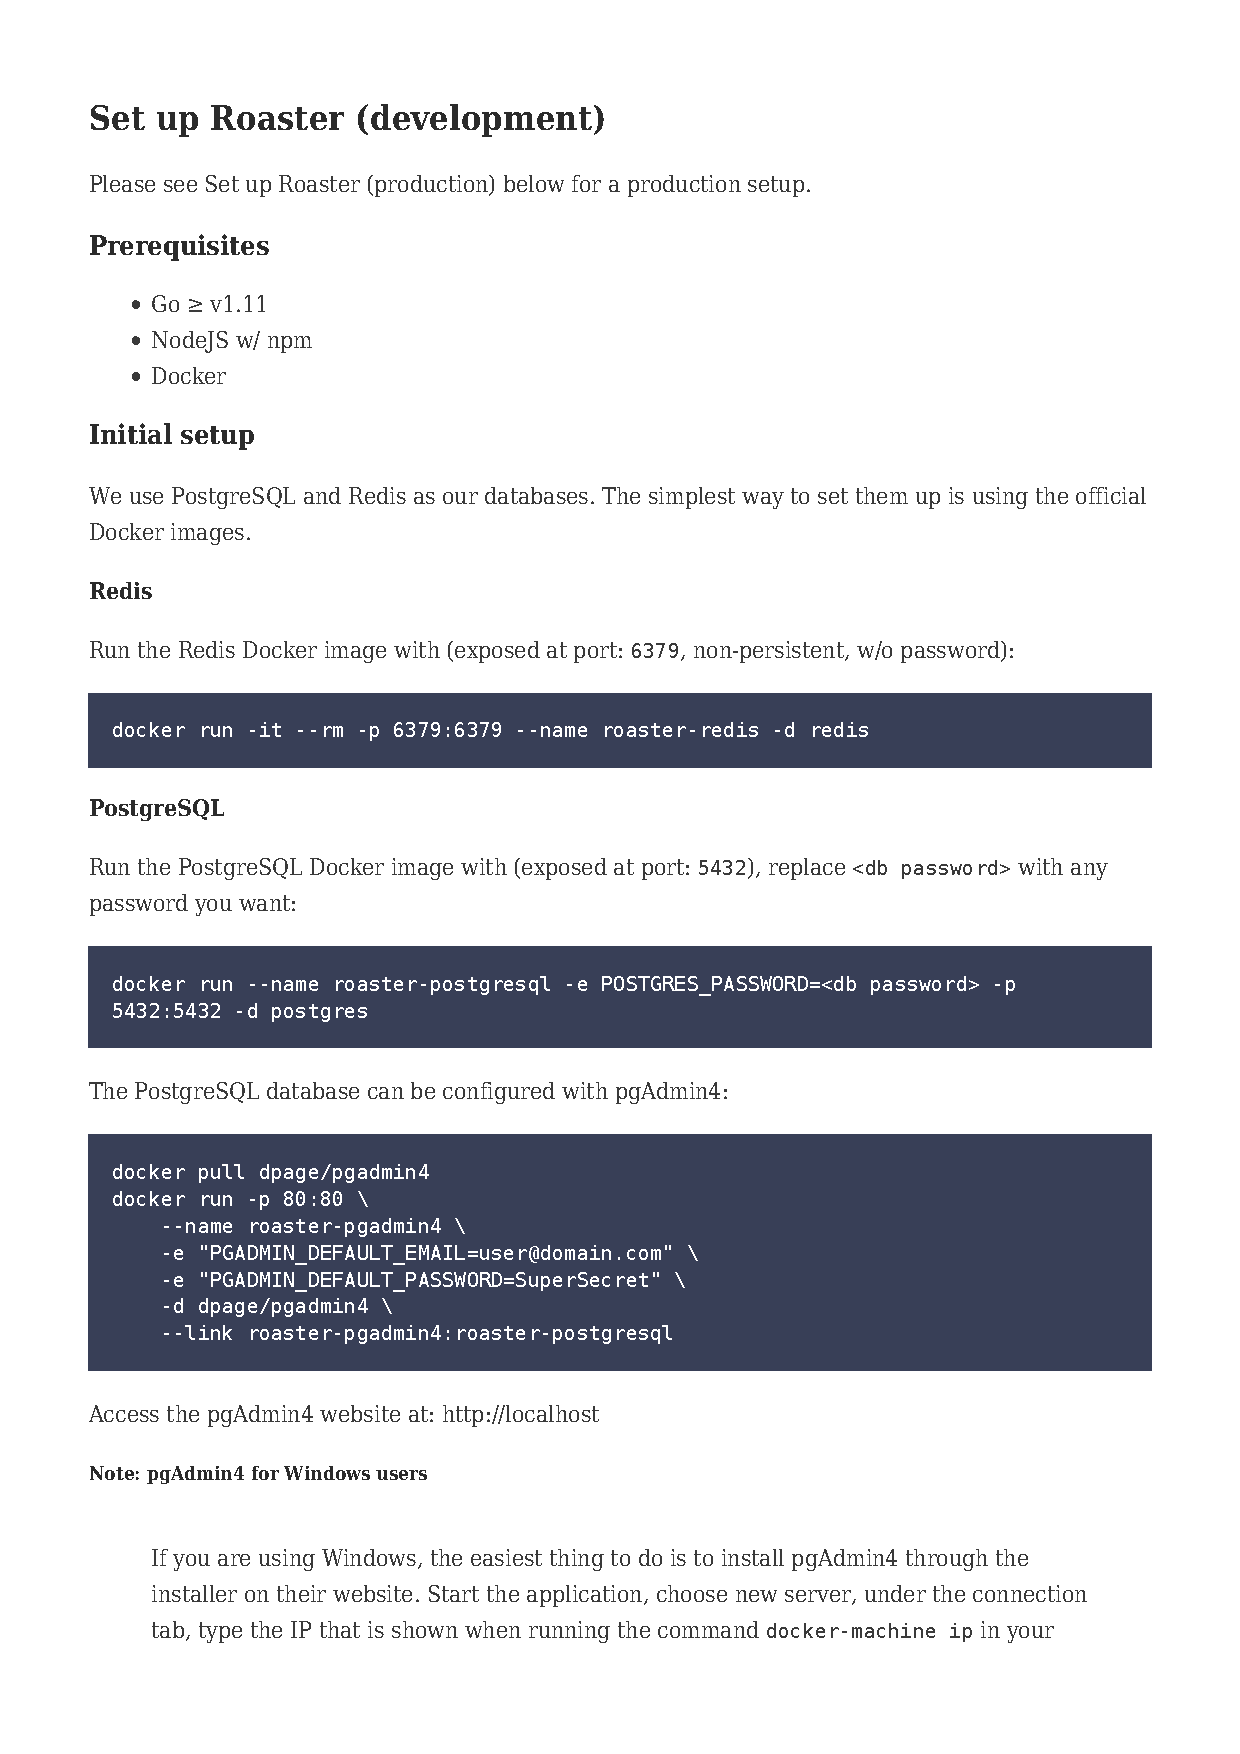
\includepdf[page=-]{install.pdf}
\end{appendix}

% Here follows some good to have examples.
\if false

\begin{figure}[H]
    \centering
    \includegraphics[width=6cm]{xxx.png}
    \caption{Lalalala.}
    \label{fig:my_label}
\end{figure}

\begin{verbatim}
PaymentTest > entitledFullAmount[ID: 505] FAILED
    java.lang.AssertionError: expected:<4960> but was:<5960>
        at org.junit.Assert.fail(Assert.java:88)
        at org.junit.Assert.failNotEquals(Assert.java:834)
        at org.junit.Assert.assertEquals(Assert.java:645)
        at org.junit.Assert.assertEquals(Assert.java:631)
        at PaymentTest.entitledFullAmount(PaymentTest.java:164)
\end{verbatim}

\begin{table}[H]
\centering
\caption{API endpoints and their methods}
\begin{tabular}{|clcl|}
\hline
\textbf{Method}              & \textbf{Endpoint}                             & \textbf{Access}              & \textbf{Description}                 \\ \hline
\multicolumn{1}{|c|}{GET}    & \multicolumn{1}{l|}{/}                        & \multicolumn{1}{c|}{N/A}     & Home page                            \\
\multicolumn{1}{|c|}{GET}    & \multicolumn{1}{l|}{/login}                   & \multicolumn{1}{c|}{N/A}     & View customer login page                      \\
\multicolumn{1}{|c|}{POST}   & \multicolumn{1}{l|}{/login}                   & \multicolumn{1}{c|}{N/A}     & Login customer user                           \\
\multicolumn{1}{|c|}{GET}    & \multicolumn{1}{l|}{/register}                & \multicolumn{1}{c|}{N/A}     & View customer register page                   \\
\multicolumn{1}{|c|}{POST}   & \multicolumn{1}{l|}{/register}                & \multicolumn{1}{c|}{N/A}     & Register customer user                        \\
\multicolumn{1}{|c|}{GET}    & \multicolumn{1}{l|}{/user}                    & \multicolumn{1}{c|}{C, W, A} & View user page                       \\
\multicolumn{1}{|c|}{POST}   & \multicolumn{1}{l|}{/user}                    & \multicolumn{1}{c|}{C, W, A} & Set user information                 \\
\multicolumn{1}{|c|}{GET}    & \multicolumn{1}{l|}{/article?id=\{0..n\}}     & \multicolumn{1}{c|}{C, W, A} & Get specific article by ID           \\
\multicolumn{1}{|c|}{POST}   & \multicolumn{1}{l|}{/cart}                    & \multicolumn{1}{c|}{C}       & Add artice to cart                   \\
\multicolumn{1}{|l|}{DELETE} & \multicolumn{1}{l|}{/cart?pos=\{0..n\}}       & \multicolumn{1}{c|}{C}       & Delete article from cart by position \\
\multicolumn{1}{|l|}{DELETE} & \multicolumn{1}{l|}{/cart}                    & \multicolumn{1}{c|}{C}       & Delete whole cart                    \\
\multicolumn{1}{|c|}{GET}    & \multicolumn{1}{l|}{/cart}                    & \multicolumn{1}{c|}{C}       & View cart                            \\
\multicolumn{1}{|c|}{PUT}    & \multicolumn{1}{l|}{/cart}                    & \multicolumn{1}{c|}{C}       & Order items in cart                  \\
\multicolumn{1}{|c|}{GET}    & \multicolumn{1}{l|}{/order}                   & \multicolumn{1}{c|}{W, A}    & View current orders                  \\
\multicolumn{1}{|c|}{GET}    & \multicolumn{1}{l|}{/order?id=\{0..n\}}       & \multicolumn{1}{c|}{W, A}    & View order by ID                     \\
\multicolumn{1}{|c|}{GET}    & \multicolumn{1}{l|}{/warehouse}               & \multicolumn{1}{c|}{W}       & Warehouse user home page             \\
\multicolumn{1}{|c|}{GET}    & \multicolumn{1}{l|}{/admin}                   & \multicolumn{1}{c|}{A}       & Admin user home page                 \\
\multicolumn{1}{|c|}{PUT}    & \multicolumn{1}{l|}{/order?id=\{0..n\}}       & \multicolumn{1}{c|}{W}       & Accept order by ID                   \\
\multicolumn{1}{|c|}{GET}    & \multicolumn{1}{l|}{/user?id=\{0..n\}}        & \multicolumn{1}{c|}{A}       & Display user by ID                   \\
\multicolumn{1}{|c|}{GET}    & \multicolumn{1}{l|}{/search?query=\{string\}}        & \multicolumn{1}{c|}{N/A}       & Search for article                   \\
\multicolumn{1}{|c|}{POST}   & \multicolumn{1}{l|}{/register?type=admin}     & \multicolumn{1}{c|}{A}       & Register new admin user              \\
\multicolumn{1}{|c|}{POST}   & \multicolumn{1}{l|}{/register?type=warehouse} & \multicolumn{1}{c|}{A}       & Register new warehouse user          \\
\multicolumn{1}{|c|}{POST}   & \multicolumn{1}{l|}{/register?type=customer}  & \multicolumn{1}{c|}{A}       & Register new customer user           \\ \hline
\end{tabular}
\end{table}
\fi
\end{document}
